\documentclass[UTF8,a4paper,12pt,oneside]{ctexrep}

\usepackage{geometry}
\usepackage{setspace}
\usepackage{booktabs}
\usepackage{longtable}
\usepackage{tabularx}
\usepackage{array}
\usepackage{xurl}
\usepackage{enumitem}
\usepackage{xcolor}
\usepackage{hyperref}
\usepackage{fancyhdr}
\usepackage{titlesec}
\usepackage{float}
\usepackage{graphicx}
\usepackage{listings}

\geometry{left=2.8cm,right=2.8cm,top=2.8cm,bottom=2.8cm}
\onehalfspacing
\setlength{\parindent}{2em}
\setlength{\parskip}{0.28em}
\setlist[itemize]{leftmargin=2.3em,itemsep=0.2em}
\setlist[enumerate]{leftmargin=2.6em,itemsep=0.2em}

\setCJKmainfont{NotoSerifCJKsc-Regular.otf}[
  Path = ./font/,
  BoldFont = NotoSerifCJKsc-Bold.otf
]

\setmonofont{consola.ttf}[
  Path = ./font/,
  BoldFont = consolab.ttf,
  ItalicFont = consolai.ttf,
  BoldItalicFont = consolaz.ttf
]

\hypersetup{
  colorlinks=true,
  linkcolor=black,
  urlcolor=blue,
  citecolor=black,
  pdfauthor={seccomp-privacy-platform team},
  pdftitle={面向电商隐私分析场景的 SSE + PJC 平台设计与实现}
}

\pagestyle{fancy}
\setlength{\headheight}{15pt}
\fancyhf{}
\fancyhead[C]{面向电商隐私分析场景的 SSE + PJC 平台设计与实现}
\fancyfoot[C]{\thepage}
\renewcommand{\headrulewidth}{0.4pt}

\ctexset{
  chapter = {
    name = {第,章},
    number = \chinese{chapter},
    format = \centering\zihao{3}\heiti,
    beforeskip = 12pt,
    afterskip = 18pt
  },
  section = {
    format = \zihao{4}\heiti,
    beforeskip = 12pt,
    afterskip = 6pt
  },
  subsection = {
    format = \zihao{-4}\heiti,
    beforeskip = 8pt,
    afterskip = 4pt
  }
}

\lstset{
  basicstyle=\ttfamily\small,
  breaklines=true,
  frame=single,
  columns=fullflexible,
  keepspaces=true,
  backgroundcolor=\color{gray!5}
}

\newcommand{\project}{seccomp-privacy-platform}
\newcommand{\pipeline}{metadata/control-plane $\rightarrow$ SSE $\rightarrow$ recovery $\rightarrow$ bridge $\rightarrow$ PJC $\rightarrow$ release}
\newcommand{\filepath}[1]{\path{#1}}
\newcommand{\figplaceholder}[2]{
  \begin{figure}[H]
    \centering
    \fbox{
      \begin{minipage}[c][0.28\textheight][c]{0.86\textwidth}
        \centering
        \vspace{0.6em}
        {\heiti 待补充图片}\\[0.8em]
        #1\\[0.8em]
        {\small 建议使用白色或浅色背景，避免大面积红色、黑色和强烈渐变。}
        \vspace{0.6em}
      \end{minipage}
    }
    \caption{#2}
  \end{figure}
}

\begin{document}

\begin{titlepage}
  \centering
  \vspace*{1.5cm}
  {\zihao{2}\heiti 面向电商隐私分析场景的\\[0.3em]SSE + PJC 平台设计与实现\par}
  \vspace{2.8cm}
  {\zihao{3}\bfseries 项目结题报告\par}
  \vspace{4.8cm}
  \begin{tabular}{>{\bfseries}r l}
    作品名称： & 面向电商隐私分析场景的 SSE + PJC 平台 \\
    项目仓库： & \project \\
    作者： & 张宇杰、屈鸣成、张隽瑄 \\
    指导教师： & 付仕辉 \\
    学校/学院： & 山东大学网络空间安全学院 \\
    日期： & \today \\
  \end{tabular}
  \vfill
\end{titlepage}

\pagenumbering{Roman}

\chapter*{摘要}
\addcontentsline{toc}{chapter}{摘要}

跨平台广告归因、复购分析、风险名单交集和合规审计都需要在不同主体之间连接数据。问题在于，电商平台、广告平台、物流与服务商分别掌握用户标识、订单金额、曝光记录和履约状态，任何一方直接交换明文数据都会扩大隐私暴露面；而只依靠接口鉴权或简单哈希，又无法回答数据从哪里来、谁批准了查询、结果是否过细、重复查询是否会造成推断攻击等问题。

围绕这一现实问题，本项目设计并实现了一个面向电商隐私分析场景的 SSE + PJC 隐私计算平台。系统以控制面数据库记录租户、数据集、调用方、策略和工作流状态；以可搜索对称加密（Searchable Symmetric Encryption，SSE）完成密文候选筛选；以受控记录恢复服务从加密记录库中提取最小必要字段；以 Rust Bridge 完成 join key 规范化、作用域 HMAC 令牌化和输入承诺；最后接入 Google Private Join and Compute（PJC）完成两方集合求交和交集值聚合，并通过发布门控、隐私预算、审批流和审计链控制结果输出。

结题时，项目已经完成从候选检索、记录恢复、桥接、PJC 计算到结果发布的端到端主链路。标准示例能够得到交集数量 2、交集金额 425；Rust Bridge 完成百万级双方输入准备约 4.437 秒；PJC 百万级双方输入已通过流式路径完成计算。除主链路外，项目还实现了 typed schema、query workflow、operator console、source attestation、release gate、异常输入门禁、审计防篡改检查、外部审计锚点适配和多类 benchmark，形成了可运行、可验证、可审计的平台工程。

本项目的创新点不在于重新发明 SSE 或 PJC 协议，而在于将已有密码学组件放入一个具体的电商隐私分析执行链路中，并补齐协议落地时最容易缺失的控制面治理、输入绑定、结果发布约束和证据化验证。项目当前仍然遵循半诚实参与方和受控运维环境假设，不能声称达到恶意安全协议或完整生产级数据净室能力。后续工作应围绕恶意安全计算后端、更强 SSE 泄露缓解、真实身份根与 KMS、生产级高可用和长期运维证据继续推进。

\vspace{1em}
\noindent\textbf{关键词：} 可搜索加密；Private Join and Compute；隐私计算；电商分析；审计治理；隐私预算

\tableofcontents
\clearpage
\pagenumbering{arabic}

\chapter{作品概述}

\section{背景分析}

电商业务中的数据天然分散。广告平台更了解曝光、点击和投放计划，电商平台更了解订单、支付、复购和售后，物流与服务商掌握履约节点和服务记录。单独看任一数据域，很多分析问题都无法得到完整答案；把所有明细集中到一处，又会带来更大的隐私风险和合规风险。

以广告归因为例，广告侧希望知道某批曝光用户中有多少最终完成购买，电商侧希望验证投放转化效果，但双方都不应直接得到对方的用户清单。类似问题也出现在风险名单交集、复购人群分析、跨店铺联合统计、客服回访范围筛选等场景中。这些任务通常只需要交集数量、交集金额或阈值保护后的聚合结果，而不是交集成员的完整身份。

已有隐私计算技术为这类问题提供了基础。SSE 能在密文索引上完成关键词检索\cite{curtmola2006sse,cash2014dynamic}，Private Set Intersection 和 Private Join and Compute 能在不直接暴露集合成员的前提下完成交集统计或交集求和\cite{googlepjc,wiredpjc}，数据净室和联邦学习框架也在产业中用于跨组织数据协作\cite{awscleanrooms,fate,secretflow}。但是，底层协议本身并不能自动解决真实系统中的全部问题：谁可以发起任务、候选数据如何限定、恢复出的字段是否必要、输入是否被替换、结果是否过细、审计证据是否完整，这些都需要协议外的工程治理。

\section{项目目标}

本项目的目标不是构建一个完整电商交易系统，也不是重新设计一套新的恶意安全密码协议，而是围绕电商隐私分析任务，完成一条从数据候选筛选到结果发布的可运行平台链路。项目开始时我们把目标拆成四个层次。

第一层是隐私计算主链路。系统需要能够在不直接交换原始 join key 和业务明细的前提下，完成候选筛选、记录恢复、跨方集合求交和交集值聚合。第二层是工程服务边界。原始数据、恢复数据、桥接输入、PJC 输入和公开结果不能混在一个不可追踪的脚本里，而要拆成可独立验证的阶段。第三层是发布治理。即使 PJC 计算正确，也不代表结果一定可以发布，系统必须对小交集、重复查询、近似查询和来源不明的数据保持约束。第四层是结题可验收。每个关键阶段都应有结构化 schema、运行命令、负向测试和证据文件，能够被复现和检查。

\section{核心项目工作}

围绕上述目标，我们完成了以下工作。为避免报告只停留在功能罗列，下面按照数据在系统中的流动过程说明项目的实际建设内容。

首先，我们保留并强化了 SSE 的候选筛选能力。SSE 模块不直接给出最终分析结论，而是在加密记录和加密索引上返回候选记录标识，使后续恢复和计算都限定在必要范围内。旧版 SSE WebSocket 暴露面已经从生产路径退休，网络 pickle 类风险被门禁覆盖，核心能力收敛为候选检索和受控导出。

其次，我们把记录恢复从普通函数调用拆成独立服务边界。Record Recovery 模块负责根据候选标识恢复 join key 和必要 value 字段，支持 subprocess、Unix socket、HTTP、mTLS、请求签名、时间戳防重放、限流、最大行数、健康检查和 Prometheus 指标。这样，``能够搜索候选'' 与 ``能够读取敏感字段'' 被分离，恢复行为可以单独授权、审计和限流。

再次，我们实现了 Rust Bridge。Bridge 对 email、phone 和普通 id 做确定性规范化，再生成任务作用域内的 HMAC-SHA256 token，并输出 PJC 所需的 server/client 输入、作业元数据和输入承诺。它的作用是避免原始 join key 直接进入跨方计算，并把数据准备阶段和 PJC 执行阶段用可验证承诺连接起来。

然后，我们接入 Google Private Join and Compute 作为两方计算内核。PJC 负责在双方 token 集合上计算交集数量和交集值求和。针对大规模输入下单一 gRPC 消息大小限制，我们增加了兼容的流式路径，使百万级双方输入能够完成传输和计算。

最后，我们在协议前后补充控制面与治理层。系统实现了 metadata sidecar、query workflow、审批流、隐私预算、source attestation、release gate、audit chain、audit seal、external anchor、operator console、schema back-compat、malformed input gate 和多类 benchmark。它们共同回答一个关键问题：这次隐私计算是否只是算出了结果，还是能够证明它是在正确作用域、正确输入、正确审批和正确发布约束下得到的结果。

\section{应用前景}

本项目适合展示面向电商隐私分析的安全协作模式。广告平台与电商平台可以在不交换原始用户清单的前提下计算转化数量与成交金额；风控团队可以验证风险名单与订单人群的交集规模；合规团队可以查看任务证据、审批记录和公开摘要，而不接触底层明细。与简单 demo 相比，本项目的意义在于把隐私计算从一个单点算法扩展为一条带治理、带证据、带边界说明的工程链路。

需要明确的是，当前系统仍是竞赛版平台基线，不应被包装成完整生产级数据净室。它更像一个可运行、可解释、可验证的隐私计算平台原型，为后续接入真实身份根、真实 KMS、高可用数据库和更强安全协议提供基础。

\chapter{作品设计与实现}

本章介绍系统如何实现。为了让叙述保持清晰，我们不按照代码目录逐个展开，而按照一条隐私分析任务从提交到发布的过程说明各模块的作用。

\section{总体设计思路}

系统的主链路可以概括为：

\begin{center}
\pipeline
\end{center}

控制面首先接收查询请求，记录调用方、租户、数据集、服务、策略和审批状态。SSE 根据授权关键词或业务过滤条件完成密文候选筛选。Record Recovery 在服务边界内恢复最小必要字段。Bridge 将原始 join key 转换为任务作用域 token，并生成 PJC 输入与输入承诺。PJC 完成两方交集计算和交集值求和。Release Gate 最后检查阈值、隐私预算、审批、来源证明、输入承诺和审计证据，决定是否发布公开结果。

这一设计把“计算”和“发布”分开。PJC 解决的是如何在双方不直接交换集合成员的情况下完成交集统计；控制面解决的是谁能发起任务，数据从何而来，结果是否能发布，证据是否能被复核。这个拆分是项目的核心思路。

\begin{figure}[htbp]
  \centering
  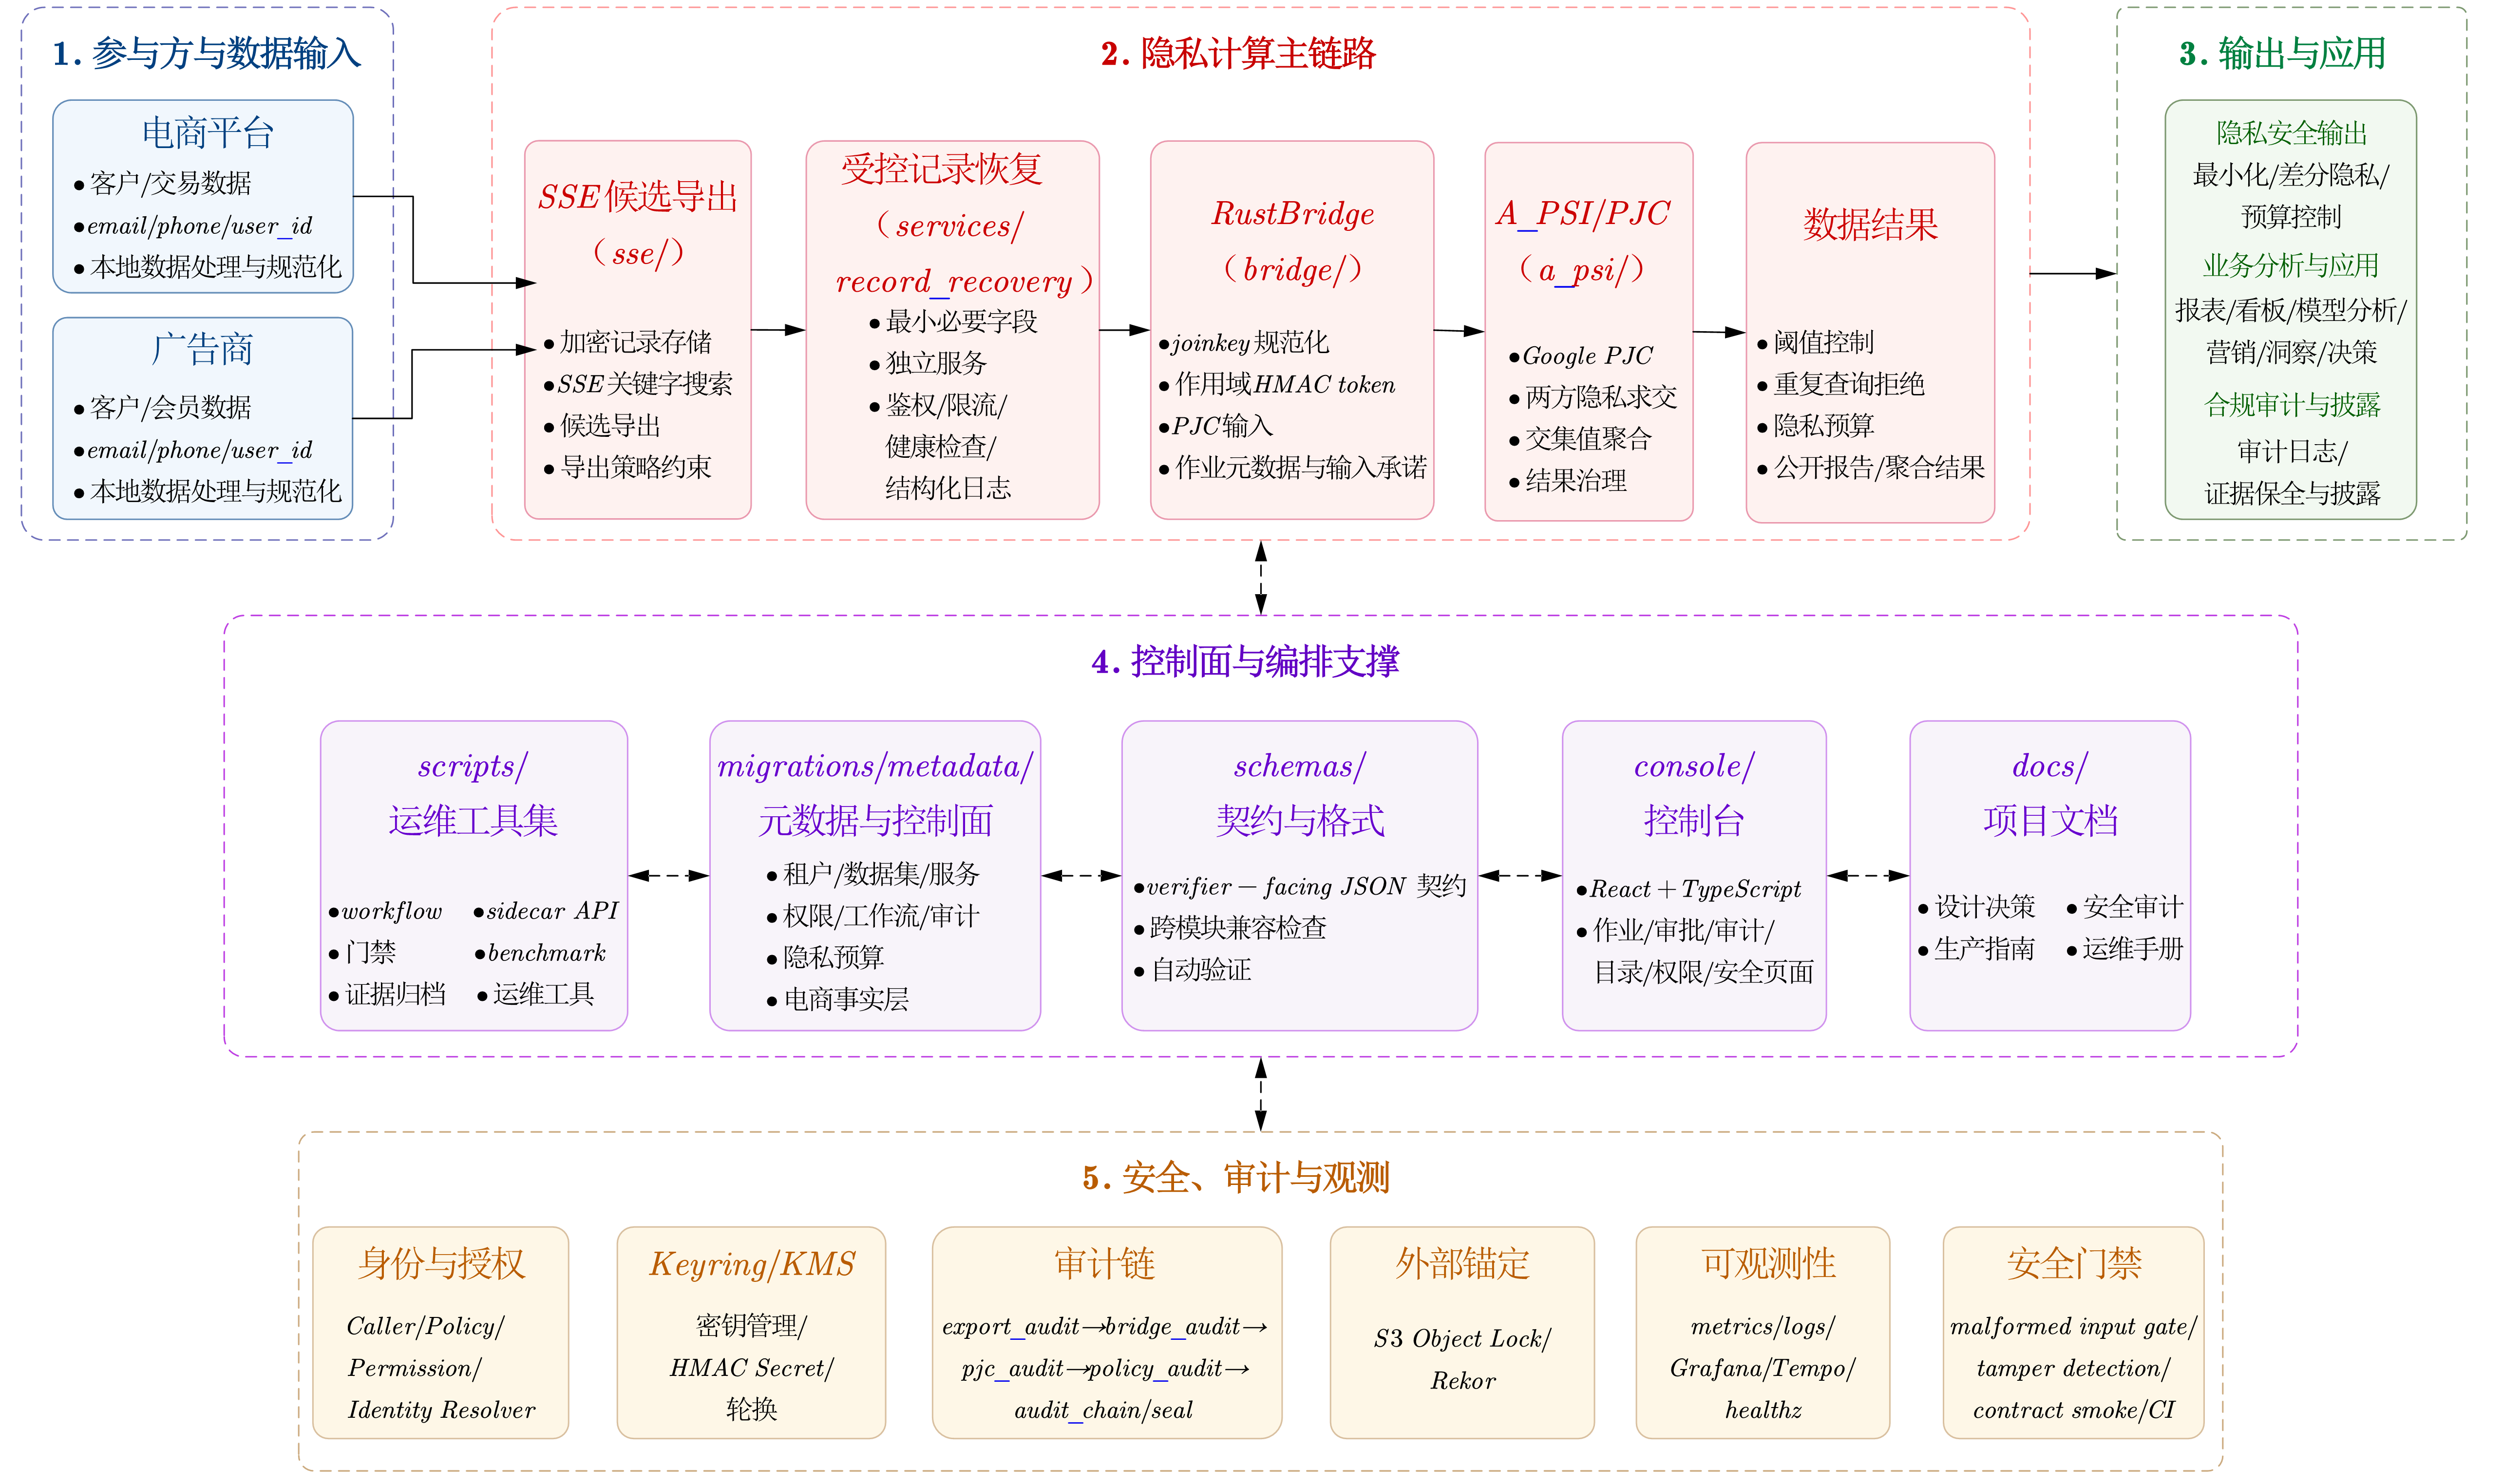
\includegraphics[width=\textwidth]{信安赛.png}
  \caption{平台总体架构图}
\end{figure}

\figplaceholder{建议补充一张重新绘制的“任务执行时序图”：从请求提交、审批、SSE 候选检索、record recovery、Bridge、PJC 到 release gate。}{隐私分析任务执行时序图（待补充）}

\section{SSE 候选筛选}

SSE 模块承担 candidate selection。它让系统能够在不直接暴露数据库明文内容的前提下，根据检索条件返回候选记录标识。候选标识本身不是最终分析结果，也不能直接用于 PJC；它只是缩小后续恢复和计算范围的第一道边界。

实现中，敏感记录被写入加密记录库，可检索字段被组织为 SSE 索引。调用方提交查询后，导出路径会检查 caller、role、join key、value field、filter field、最大导出行数和必需过滤条件。导出审计记录只保存任务、作用域、字段名、哈希和决策信息，不写入原始邮箱、手机号、设备标识或 token secret。

该模块的难点不在于简单调用搜索接口，而在于把 SSE 搜索结果放入后续治理链条。只有当候选范围、调用方身份和导出策略一致时，候选结果才会进入 record recovery 阶段。这样可以避免“能搜到”被误解为“能任意导出”。

\section{受控记录恢复}

Record Recovery 是本项目中非常关键的一层。SSE 返回的是候选标识，而 PJC 需要规范化后的 join key 和可能参与求和的 value 字段。直接让查询端读取加密记录库会破坏最小必要原则，所以我们把恢复逻辑拆成独立服务。

恢复服务使用 PBKDF2HMAC-SHA256 派生密钥，使用 AES-256-GCM 保护记录内容，并使用 keyed HMAC-SHA256 标记记录标识。服务接收候选集合后，只在授权范围内恢复必要字段，并根据配置限制调用方、租户、数据集、服务、输出目录、记录库目录和最大返回行数。HTTP 模式下，请求还要经过签名校验、时间戳防重放、caller 级限流和健康状态检查。

这一层带来的直接收益是边界清晰。候选搜索、记录恢复、桥接输入和 PJC 计算不再混在同一个脚本中；即使某个调用方获得了候选标识，也不能绕过恢复服务读取任意字段。恢复行为本身也会写入结构化审计，便于事后检查。

\section{Rust Bridge 与输入承诺}

Bridge 位于原始业务标识和 PJC 输入之间。它先对 join key 做确定性规范化，例如 email 统一大小写和空白处理，phone 统一格式；随后使用作用域绑定的 HMAC-SHA256 生成 token。作用域的存在非常重要：同一原始标识在不同任务或不同数据域中不应被简单关联。

Bridge 还会生成 PJC 作业目录、server/client 输入、作业元数据、审计事件和 input commitment。输入承诺把 Bridge 输出、关键元数据和后续 PJC 运行绑定起来。如果 Bridge 之后的 CSV、manifest 或 PJC 输入被替换，release gate 可以发现不一致。生产模式下，Bridge 不接受直接在命令行传入 token secret，而是通过环境变量、key agent 或外部 KMS adapter 获取密钥，并在审计中记录密钥来源类型而不是密钥值。

该模块解决了两个实际问题。第一，PJC 不再直接接触原始邮箱、手机号等 join key。第二，PJC 输入不再是一个难以追踪的中间文件，而是带有任务、作用域和承诺绑定的受控产物。

\section{PJC 计算}

PJC 模块负责真正的两方交集统计。系统集成 Google Private Join and Compute，采用双方 token 集合作为输入，计算交集大小以及交集上 client value 的聚合值。典型场景中，广告侧作为 server 提供曝光集合，电商侧作为 client 提供转化用户与金额，最终得到交集数量和交集金额。

在工程实现上，项目提供了 server/client 运行脚本、TLS 与 mTLS 配置、分桶分片流程、结果合并、输入承诺检查和发布前验证。针对百万级输入，原始 gRPC 路径会受到消息大小限制，因此我们增加了流式传输路径，将大规模重复加密集合按块传输，最终完成百万级双方输入测试。

需要强调的是，PJC 的安全边界仍然是半诚实参与方模型。输入承诺和来源证明能够发现 repo-side 路径中的替换和无证据运行，但不能阻止一方主动偏离协议、伪造源数据或提交异常 value。这个边界在报告中必须讲清楚，否则会给评委留下夸大安全性的印象。

\section{控制面、工作流与操作台}

控制面是本项目从“算法 demo”走向“平台工程”的主要部分。Metadata sidecar 使用 SQLite/PostgreSQL 双后端记录租户、数据集、服务、调用方、权限、策略、密钥注册、作业状态、审计事件和隐私预算。它不承担完整电商事实库职责，而是回答：谁在什么作用域下发起了什么任务，经过哪些阶段，哪些阶段允许或拒绝，产生了哪些证据。

Query Workflow 将请求提交、审核、批准、入队、worker 执行、结果发布和状态回写连接起来。审批流程禁止同一身份自批，隐私预算使用事务化存储，避免并发条件下同一预算被重复消费。Operator Console 则提供作业、请求、审计、目录、权限、恢复服务、可观测性、合规和安全页面，使平台不仅能通过命令行运行，也能通过操作面展示完整过程。

\chapter{项目完成情况与成果}

结题报告的重点应当回答“最终做成了什么”。本章将项目成果从主链路、平台能力、验证结果和团队工作量四个角度进行总结。

\section{完成的主链路}

项目最终完成了从密文候选检索到受控结果发布的完整链路。标准任务中，系统可以从 SSE 检索候选记录，经 record recovery 恢复最小必要字段，由 Bridge 生成 PJC 输入，再通过 PJC 得到交集数量和交集金额，最后由 release gate 输出公开报告。标准示例结果为 \texttt{intersection\_size=2}，\texttt{intersection\_sum=425}。

这条链路的完成意义不只是“跑通了一个脚本”。每个阶段都有输入输出契约、审计记录和失败路径：SSE 阶段有导出策略，恢复阶段有服务授权和限流，Bridge 阶段有 tokenization 和 input commitment，PJC 阶段有运行证据，release 阶段有阈值、预算和证据检查。它们共同构成了一个可复核的执行闭环。

\section{完成的平台能力}

\begin{longtable}{p{0.26\textwidth}p{0.64\textwidth}}
\caption{项目主要完成成果}\\
\toprule
\textbf{成果类别} & \textbf{具体完成内容} \\
\midrule
\endfirsthead
\toprule
\textbf{成果类别} & \textbf{具体完成内容} \\
\midrule
\endhead
\bottomrule
\endfoot
隐私计算主链路 & 完成 \pipeline{} 主链路，支持标准 demo、文件交接、FIFO 交接、record recovery 服务路径和 PJC 发布路径。 \\
服务边界 & 将记录恢复拆分为独立服务，支持 Unix socket、HTTP、mTLS、请求签名、防重放、限流、健康检查和指标暴露。 \\
Bridge 工程 & 使用 Rust 实现 join key 规范化、作用域 HMAC token、PJC 输入生成、审计记录和 input commitment。 \\
发布治理 & 实现 release gate、privacy budget、approval workflow、source attestation、release governance report 和外部审计锚点适配。 \\
控制面 & 实现 metadata sidecar、query workflow、operator dashboard、业务身份注解、权限模型和 read-only API。 \\
验证体系 & 建立 JSON Schema、schema back-compat、contract smoke、CI smoke、负向安全测试、benchmark 和 live evidence gate。 \\
展示界面 & 完成基于 Vite、React、TypeScript 的 operator console，覆盖作业、请求、审计、目录、权限、恢复、可观测性和安全页面。 \\
\end{longtable}

\section{关键实验结果}

项目验证分为功能验证、安全验证和性能验证。功能验证关注主链路是否能够得到正确结果；安全验证关注恶意输入、重放、篡改和越权路径是否被拒绝；性能验证关注 SSE、record recovery、Bridge、PJC 和完整管线在不同规模下的资源表现。

\begin{longtable}{p{0.30\textwidth}p{0.58\textwidth}}
\caption{关键验证结果汇总}\\
\toprule
\textbf{验证项} & \textbf{结果摘要} \\
\midrule
\endfirsthead
\toprule
\textbf{验证项} & \textbf{结果摘要} \\
\midrule
\endhead
\bottomrule
\endfoot
标准端到端示例 & 得到交集数量 2、交集金额 425，主链路结果与预期一致。 \\
顶层闭环状态 & 16 个 verifier-facing 模块达到 repo-side 与 live-side 状态为 ok，live fail 为 0。 \\
SSE Export 规模 & 完成 100k 和 1M candidates 本地规模测试。 \\
Record Recovery & 1k candidates、10 路 HTTP 并发测试吞吐为 15.818 req/s。 \\
Rust Bridge & 100k/100k 输入约 0.366 秒；1M/1M 输入约 4.437 秒。 \\
PJC 规模 & 100k/100k 测试约 222.02 秒；流式 1M/1M 测试约 34 分 05 秒，峰值 RSS 约 2.20 GB。 \\
完整管线 & 10k 规模完整管线约 34.9 秒，结果与预期一致。 \\
安全负向测试 & malformed HTTP 输入、错误签名、重放、网络 pickle、审计 bit-flip 篡改等均有自动门禁。 \\
\end{longtable}

这些结果说明，项目已经不是单一算法验证，而是完成了一套可执行、可测量、可审计的平台化实现。同时，性能结果也暴露出明确边界：SSE Export 资源需求较轻，PJC 对地址空间、双进程通信和密钥生成更敏感，后续部署需要单独规划 PJC 资源隔离和任务调度。

\figplaceholder{建议补充浅色版“项目完成成果总览图”：用一张图展示主链路、控制面、验证体系和展示界面四类成果。}{项目完成成果总览图（待补充）}

\figplaceholder{建议补充浅色版“SSE 与 PJC 资源实验图”：不要使用红色背景或黑色 FAIL 区域；失败区域建议用浅灰和斜线表示。}{SSE 与 PJC 资源实验结果图（待替换旧图）}

\section{团队收获}

通过本项目，我们最大的收获不是学会调用某一个密码学库，而是理解了隐私计算系统落地时的复杂性。底层协议只解决一部分问题，真实系统还必须处理数据来源、权限边界、密钥来源、失败路径、审计证据、性能资源和人机操作流程。没有这些工程治理，隐私计算很容易停留在“能算但不可用、可用但不可管、可管但不可证”的状态。

在工程能力上，团队完成了 Python、Rust、TypeScript、Shell、SQL、JSON Schema 和多类服务接口的协作开发；在安全理解上，团队区分了协议内安全和协议外治理，避免把半诚实 PJC 误称为恶意安全；在测试意识上，团队从只验证成功路径，扩展到验证恶意输入、重放、篡改、资源失败和 schema 兼容性。这些收获比单个 benchmark 数字更重要，因为它们决定了项目是否能够被解释、复现和继续演进。

\chapter{测试与分析}

\section{测试方法}

项目采用分层测试方法。最底层是 schema 和编译检查，保证各模块产物符合冻结契约。中间层是模块 smoke 和负向测试，验证 SSE、record recovery、Bridge、PJC、release gate 和 sidecar API 的行为。最上层是端到端 demo、benchmark、live evidence 和 closure gate，用于证明主链路与平台证据能够整体收口。

常用验证入口包括：

\begin{lstlisting}[language=bash]
bash scripts/run_live_sse_bridge_demo.sh
bash scripts/check_json_contracts.sh
bash scripts/check_ci_smoke.sh
python3 scripts/check_schema_backcompat.py
python3 scripts/check_http_malformed_input_gate.py
python3 scripts/verify_audit_tamper_resistance.py --help
python3 scripts/benchmark_smoke.py --help
\end{lstlisting}

\section{功能测试分析}

功能测试以完整主链路为核心。系统从示例电商数据出发，执行 SSE 候选检索、record recovery、Bridge tokenization、PJC 计算和 release gate 发布，最终得到交集数量 2 和交集金额 425。这个结果本身并不复杂，但它证明了多模块之间的输入输出契约已经对齐。

在此基础上，query workflow 和 operator console 进一步验证了平台操作路径。任务不再只能由单个脚本直接触发，而可以经过请求提交、审批、执行和状态回写。审计 API、platform health API 和 public report 也能为展示和复核提供结构化结果。

\section{安全测试分析}

安全测试重点覆盖失败路径。HTTP recovery service 会拒绝缺失签名、错误签名、过期时间戳、未来时间戳、坏 JSON、非对象 payload、未知路径、错误方法和超大 body。Audit tamper resistance 测试会对审计链和 seal 做 bit-flip，验证篡改能够被发现。Legacy SSE WebSocket 的网络 pickle 风险已经通过生产门禁退休，不再作为生产查询面。

这些测试不能证明系统达到恶意安全，但能证明项目对常见工程风险不是无感的。对竞赛项目而言，这一点很关键：一个只展示成功路径的隐私计算 demo 很容易掩盖真实风险，而本项目将失败路径也纳入了验收范围。

\section{性能测试分析}

性能测试显示，SSE Export 与 PJC 的资源特征差异明显。SSE Export 在当前规模下工作集较小，20,000 candidates 测试中峰值 RSS 稳定在约 43 MB，增加 CPU 核数和内存容量没有带来稳定线性加速，说明瓶颈更多来自单进程处理、记录读取和输出写入。

PJC 对资源更加敏感。在 1,000 $\times$ 1,000 双方输入资源矩阵中，低内存区域出现大量失败点；约 1.5 GB 地址空间后稳定性明显改善。百万级双方输入虽然已经通过流式路径完成，但耗时仍达到 34 分 05 秒，说明 PJC 需要单独的资源规划、分片并行、超时控制和失败重试策略。

因此，后续部署不能把 SSE 和 PJC 当成同一种负载处理。SSE 更适合轻量候选筛选和批量调度，PJC 更像资源敏感型计算任务，应当放入独立 worker、资源限额和队列调度中。

\chapter{创新性说明}

\section{创新性边界}

必须先明确边界：本项目没有发明新的 SSE 原语，也没有发明新的 PJC 协议。SSE、PSI-SUM、HMAC、AES-GCM、PBKDF2、OIDC、OpenFGA 风格授权和数据净室思想都有成熟研究或工程实现。把这些已有概念简单堆在一起，不能称为强创新。

本项目的创新性主要体现在系统组合、执行链路和治理闭环上。也就是说，我们的工作重点不是“提出一个全新的密码算法”，而是“让已有密码学能力在一个具体电商隐私分析场景中可运行、可约束、可审计、可复核”。

\section{端到端链路创新}

传统 PJC demo 往往从双方 CSV 输入开始，直接运行交集求和。真实电商场景中，输入不会天然以干净 CSV 形式存在，敏感字段也不能随意导出。因此，本项目在 PJC 前加入 SSE candidate selection 和 controlled record recovery，使 PJC 输入来自受控候选集合和最小必要字段。

这条链路的创新点在于分层约束。SSE 限定候选范围，record recovery 限定明文字段，Bridge 限定 join key 表达，PJC 限定跨方计算，release gate 限定最终输出。每一层只做自己该做的事，并留下证据给下一层检查。

\section{Bridge 与输入绑定创新}

Bridge 并不是普通格式转换脚本。它把原始 join key 转换为作用域 HMAC token，并生成 PJC 输入承诺。这样，原始邮箱或手机号不会直接进入 PJC，任务之间的 token 也不能被简单关联；同时，Bridge 输出被绑定到作业元数据和后续 release gate，减少中间文件被替换的空间。

这一设计补上了很多隐私计算 demo 的薄弱环节：协议本身可能是安全的，但输入准备阶段经常没有同等强度的约束。本项目把输入准备阶段纳入了治理链条。

\section{发布治理创新}

隐私计算的结果并不天然安全。即使双方没有交换原始集合，小交集、重复查询、近似查询和交集求和仍可能造成推断风险。项目通过 release gate、privacy budget、approval workflow、source attestation 和 external anchor 控制结果发布，使“算出结果”和“允许发布”成为两个不同判断。

这种设计借鉴了数据净室和隐私预算的思想，但没有依赖某个云厂商托管平台。它以本地可运行代码、JSON Schema 和审计证据实现，适合竞赛展示和复核。

\section{与已有工作的比较}

\begin{longtable}{p{0.23\textwidth}p{0.31\textwidth}p{0.34\textwidth}}
\caption{本项目与已有工作的比较}\\
\toprule
\textbf{已有工作} & \textbf{主要能力} & \textbf{本项目的差异} \\
\midrule
\endfirsthead
\toprule
\textbf{已有工作} & \textbf{主要能力} & \textbf{本项目的差异} \\
\midrule
\endhead
\bottomrule
\endfoot
Google Private Join and Compute & 提供两方 Private Join and Compute / PSI-SUM 能力，适合交集统计和交集求和。 & 本项目没有重写 PJC，而是在其前后增加 SSE 候选筛选、record recovery、Bridge tokenization、input commitment、release gate 和审计证据链。 \\
SSEPy 与典型 SSE 方案 & 提供加密索引和密文关键词检索能力。 & 本项目把 SSE 定位为 PJC 前的 candidate selection，而不是单独文件检索 demo，并将候选导出纳入权限和审计。 \\
AWS Clean Rooms 等数据净室产品 & 提供托管式跨组织数据协作、规则约束和审计能力。 & 本项目是竞赛版开源工程实现，突出 SSE + PJC + 控制面治理的可运行链路，而不是云厂商托管服务。 \\
FATE、SecretFlow 等隐私计算框架 & 面向联邦学习、MPC、隐私保护数据分析和机器学习。 & 本项目不主打模型训练，而聚焦电商交集分析、结果发布治理和 verifier-facing evidence。 \\
\end{longtable}

因此，本项目应当把创新点讲成“系统化集成与治理增强”，而不是“底层协议原创”。这种表述更准确，也更经得起专业评审追问。

\chapter{不足与改进方向}

\section{当前不足}

项目已经完成竞赛版平台基线，但仍有清晰边界。

第一，PJC 仍基于半诚实参与方模型，不能阻止恶意参与方主动偏离协议、伪造源数据或提交异常 value。第二，SSE 仍会泄露搜索模式、访问模式和候选规模，当前没有采用 ORAM、forward-private SSE 或 OPRF-blinded query。第三，百万级 PJC 虽然已经通过流式路径完成，但耗时和资源需求仍偏高。第四，真实身份根、KMS、不可变审计锚点、PostgreSQL 高可用和长期 SRE 流程不是代码仓库自身能够完全替代的。第五，电商事实层和业务身份模型仍是适配基线，还不是完整的业务中台。

\section{不更换主线时的改进}

在不替换现有 SSE + PJC 主线的前提下，后续可以继续做四类改进。

一是增强 release gate，对跨任务差分、相近时间窗口、阈值探测和异常 value 提供更细粒度检测。二是完善 workflow 持久性，引入真实 PostgreSQL、队列和 worker 生命周期管理，使任务恢复、重试和失败补偿更加稳定。三是提升 PJC 性能，采用分桶并行、连接复用、密钥生成优化和资源隔离，降低大规模任务的尾延迟。四是补齐生产证据，在真实 OIDC、OpenFGA、Vault、cloud KMS、mTLS、S3 Object Lock 或 Rekor 环境中持续收集 live evidence。

\section{需要超出当前框架的问题}

如果要抵抗恶意计算参与方，仅靠当前 input commitment 和 source attestation 不够，需要接入 malicious-secure PSI-SUM、主动安全 MPC/2PC、零知识范围证明、值证明或可信执行环境。若要显著降低 SSE 访问模式泄露，需要采用 ORAM、forward-private SSE、OPRF 盲化查询等更强方案。若要形成真正生产级数据净室，还需要长期运营的企业身份根、密钥管理、审计机构、不可变存储和高可用基础设施。

\chapter{总结}

本项目围绕电商隐私分析中的跨方集合匹配和聚合计算问题，完成了一个由控制面数据库、SSE 候选筛选、受控记录恢复、Rust Bridge、Google PJC 和发布治理组成的隐私计算平台。项目不仅跑通了端到端计算链路，还把权限、输入承诺、来源证明、隐私预算、审批流、审计链、外部锚点和自动化验证纳入同一工程体系。

从结题成果看，项目已经能够完成标准隐私分析任务，得到可复现的交集数量和交集金额；能够在百万级输入上完成 Bridge 准备和 PJC 流式计算；能够通过 schema、smoke、负向测试和 benchmark 证明关键模块行为。与普通算法 demo 相比，本项目更强调隐私计算落地时的过程治理和证据化交付。

从团队收获看，我们认识到隐私计算系统不能只关注协议本身。一个可信的平台还需要清晰的服务边界、密钥边界、权限边界、发布边界和审计边界。项目当前仍有半诚实模型、SSE 泄露、生产信任根和性能扩展方面的限制，但这些限制已经被明确记录，并为后续改进提供了方向。

总的来说，本项目完成了竞赛阶段的主要目标：将已有密码学组件和工程控制面结合起来，形成一个面向电商隐私分析场景的可运行、可治理、可审计平台基线。

\appendix

\chapter{建议补充的图片清单}

为了提升报告表达效果，建议后续补充或替换以下图片：

\begin{enumerate}
  \item \textbf{任务执行时序图：}展示请求提交、审批、SSE、record recovery、Bridge、PJC、release gate 和审计归档的时序关系。
  \item \textbf{项目完成成果总览图：}用一张浅色图展示主链路、控制面、验证体系和展示界面。
  \item \textbf{浅色版 SSE 资源热力图：}原图大面积红色，建议改为蓝色或绿色顺序色标。
  \item \textbf{浅色版 PJC 资源热力图：}原图大面积黑色 FAIL，建议用浅灰斜线表示失败区，并把标题改为“资源不足未完成区域”。
  \item \textbf{Operator Console 截图：}选择 jobs、requests、audit 或 security 页面，证明系统有可展示的操作面。
\end{enumerate}

\chapter{主要验证命令}

\begin{lstlisting}[language=bash]
# 端到端主链路
bash scripts/run_live_sse_bridge_demo.sh

# JSON 契约与 CI smoke
bash scripts/check_json_contracts.sh
bash scripts/check_ci_smoke.sh
python3 scripts/check_schema_backcompat.py

# 安全负向测试
python3 scripts/check_http_malformed_input_gate.py
python3 scripts/verify_audit_tamper_resistance.py --help

# Benchmark 入口
python3 scripts/benchmark_smoke.py --help
python3 scripts/benchmark_pjc.py --help
\end{lstlisting}

\begin{thebibliography}{99}

\bibitem{curtmola2006sse}
R. Curtmola, J. Garay, S. Kamara, and R. Ostrovsky.
Searchable Symmetric Encryption: Improved Definitions and Efficient Constructions.
In \textit{ACM CCS}, 2006.

\bibitem{cash2014dynamic}
D. Cash, J. Jaeger, S. Jarecki, C. Jutla, H. Krawczyk, M.-C. Rosu, and M. Steiner.
Dynamic Searchable Encryption in Very-Large Databases: Data Structures and Implementation.
In \textit{NDSS}, 2014.

\bibitem{googlepjc}
Google.
Private Join and Compute.
\url{https://github.com/google/private-join-and-compute}.

\bibitem{wiredpjc}
L. Newman.
Google Turns to Retro Cryptography to Keep Data Sets Private.
\textit{Wired}, 2019.
\url{https://www.wired.com/story/google-private-join-compute-database-encryption/}.

\bibitem{awscleanrooms}
Amazon Web Services.
AWS Clean Rooms.
\url{https://aws.amazon.com/clean-rooms/}.

\bibitem{fate}
FederatedAI.
FATE: An Industrial Grade Federated Learning Framework.
\url{https://github.com/FederatedAI/FATE}.

\bibitem{secretflow}
SecretFlow.
SecretFlow: A Unified Framework for Privacy-Preserving Data Intelligence and Machine Learning.
\url{https://github.com/secretflow/secretflow}.

\bibitem{nistgcm}
M. Dworkin.
Recommendation for Block Cipher Modes of Operation: Galois/Counter Mode (GCM) and GMAC.
NIST Special Publication 800-38D, 2007.

\bibitem{rfc2104}
H. Krawczyk, M. Bellare, and R. Canetti.
HMAC: Keyed-Hashing for Message Authentication.
RFC 2104, 1997.

\bibitem{rfc8018}
K. Moriarty, B. Kaliski, and A. Rusch.
PKCS \#5: Password-Based Cryptography Specification Version 2.1.
RFC 8018, 2017.

\end{thebibliography}

\end{document}
